\documentclass[convert, border=2pt,outext=.png]{standalone}

\usepackage[utf8]{inputenc}
\usepackage{lmodern}
\usepackage[T1]{fontenc}

\usepackage{bm}

\usepackage[europeanvoltages, europeancurrents, europeanresistors]{circuitikz}

\usepackage{tikz}
\usetikzlibrary{positioning}
\usetikzlibrary{arrows,arrows.meta}
\usetikzlibrary{decorations,decorations.markings,decorations.pathreplacing,decorations.pathmorphing}
\usetikzlibrary{calc,math}
\usetikzlibrary{patterns}
\usetikzlibrary{shapes,shapes.symbols}

\tikzstyle{block} = [draw, fill=white, rectangle, minimum height=3em, minimum width=4em]
\tikzstyle{rblock} = [draw, fill=white, circle, inner sep=0pt,minimum size=1mm]
\tikzstyle{wobblock} = [fill=white, rectangle, minimum height=3em, minimum width=5em]
\tikzstyle{nlblock} = [draw, postaction={draw,line width=0.25mm,white}, line width=0.5mm, black, fill=white, rectangle, minimum height=3em, minimum width=5em]
\tikzstyle{sum} = [draw,circle]
\tikzstyle{branch} = [circle,inner sep=0pt,minimum size=1mm,fill=black,draw=black]
\tikzstyle{nvbranch} = [circle,inner sep=0pt,minimum size=1mm,fill=white,draw=white, fill opacity=0, draw opacity=0]
\tikzstyle{vecBranch} = [circle,inner sep=0pt,minimum size=2mm,fill=black,draw=black]
\tikzstyle{input} = [coordinate]
\tikzstyle{output} = [coordinate]
\tikzstyle{coord} = [coordinate]
\tikzstyle{pinstyle} = [pin edge={<-,thin,black,>=latex'}]

\newcommand{\uS}[1][non]{\ensuremath{\ifthenelse{\equal{#1}{non}}{u_{\mathrm{S}}}{u_{\mathrm{S,#1}}}}}
\newcommand{\uR}[1][non]{\ensuremath{\ifthenelse{\equal{#1}{non}}{u_{\mathrm{R}}}{u_{\mathrm{R,#1}}}}}
\newcommand{\bmw}[1][non]{\ensuremath{\ifthenelse{\equal{#1}{non}}{\bm{w}}{\bm{w}_{\mathrm{#1}}}}}
\newcommand{\bmd}[1][non]{\ensuremath{\ifthenelse{\equal{#1}{non}}{\bm{d}}{\bm{d}_{\mathrm{#1}}}}}

\newcommand{\Ain}[1][non]{\ensuremath{\ifthenelse{\equal{#1}{non}}{A_{\mathrm{zu}}}{A_{\mathrm{zu, #1}}}}}
\newcommand{\Aout}[1][non]{\ensuremath{\ifthenelse{\equal{#1}{non}}{A_{\mathrm{ab}}}{A_{\mathrm{ab, #1}}}}}
\newcommand{\uA}[1][non]{\ensuremath{\ifthenelse{\equal{#1}{non}}{u_{\mathrm{A}}}{u_{\mathrm{A, #1}}}}}
\newcommand{\buA}[1][non]{\ensuremath{\ifthenelse{\equal{#1}{non}}{\bar{u}_{\mathrm{A}}}{\bar{u}_{\mathrm{A, #1}}}}}
\newcommand{\AT}[1][non]{\ensuremath{\ifthenelse{\equal{#1}{non}}{A_{\mathrm{T}}}{A_{\mathrm{T, #1}}}}}
\newcommand{\hv}[1][non]{\ensuremath{\ifthenelse{\equal{#1}{non}}{h_{\mathrm{V}}}{h_{\mathrm{V, #1}}}}}
\newcommand{\hvb}[1][non]{\ensuremath{\ifthenelse{\equal{#1}{non}}{\bar{h}_{\mathrm{V}}}{\bar{h}_{\mathrm{V, #1}}}}}
\newcommand{\Vd}[1][non]{\ensuremath{\ifthenelse{\equal{#1}{non}}{\dot{V}_{}}{\dot{V}_{#1}}}}
\newcommand{\Vdin}[1][non]{\ensuremath{\ifthenelse{\equal{#1}{non}}{\dot{V}_{\mathrm{zu}}}{\dot{V}_{\mathrm{zu, #1}}}}}
\newcommand{\Vdout}[1][non]{\ensuremath{\ifthenelse{\equal{#1}{non}}{\dot{V}_{\mathrm{ab}}}{\dot{V}_{\mathrm{ab, #1}}}}}
\newcommand{\ub}[1][non]{\ensuremath{\ifthenelse{\equal{#1}{non}}{\bar{u}}{\bar{u}}}}
\newcommand{\Ku}{\ensuremath{K_{\mathrm{U}}}}
\newcommand{\dz}{\ensuremath{\dot{z}}}
\newcommand{\tdz}{\ensuremath{\dot{\tilde{z}}}}
\newcommand{\Vpos}[1][non]{\ensuremath{\ifthenelse{\equal{#1}{non}}{V_{\mathrm{pos}}}{V_{\mathrm{pos, #1}}}}}
\newcommand{\dVT}{\ensuremath{\dot{V}_{\mathrm{T}}}}
\newcommand{\Fw}[1][non]{\ensuremath{\ifthenelse{\equal{#1}{non}}{F_{\mathrm{w}}}{F_{\mathrm{w, #1}}}}}
\newcommand{\Fg}[1][non]{\ensuremath{\ifthenelse{\equal{#1}{non}}{F_{\mathrm{g}}}{F_{\mathrm{g, #1}}}}}
\newcommand{\aus}[1][non]{\ensuremath{\ifthenelse{\equal{#1}{non}}{a_{\mathrm{US}}}{a_{\mathrm{US, #1}}}}}
\newcommand{\bus}[1][non]{\ensuremath{\ifthenelse{\equal{#1}{non}}{b_{\mathrm{US}}}{b_{\mathrm{US, #1}}}}}

\newif\ifHVAC
\newif\ifHVACCtrl
\newif\ifAddQ

\begin{document}
    % Raumklimatisierung
    \HVACtrue
    \HVACCtrltrue
    \AddQtrue
%	\tikzset{
    person/.pic={
        \draw[thick,fill=white] (-0.35*2,2) circle (0.15*2) coordinate (H);
        \draw[thick] (H)++(-90:0.15*2) coordinate (N) to[out=-95,in=95]++ (0,-0.40*2) coordinate (P);
        \draw[thick,line cap=round] (N)++(-95:0.03) to[out=-60,in=95]++ (0.10*2,-0.4*2) coordinate (RH);
        \draw[thick,line cap=round] (N)++(-95:0.03) to[out=-120,in=90]++ (-0.08*2,-0.4*2);
        \draw[thick] (P) to[out=-70,in=95] ($(H)+(0.08*2,-2)$);
        \draw[thick] (P) to[out=-100,in=72] ($(H)+(-0.08*2,-2)$);
    }
}
\tikzset{
    sunflames/.style={
        line width=1pt,
        draw=orange!85,
        fill=orange!85,
        regular polygon,
        regular polygon sides=3,
        inner sep=0.075cm
    },
    sunbody/.style={
        line width=2pt,
        draw=orange!85,
        fill=orange!85,
        circle,
        minimum size=0.65cm
    }
}

\newcommand{\TwoCol}[3][A]{%
  \begin{tikzpicture}
    \begin{scope}
      \node[inner sep=0.1pt,outer sep=0.1pt] (a) {\phantom{#1}};
      \clip (a.south west) rectangle ($(a.north)-(0.5\pgflinewidth,0)$);
      \node[inner sep=0.1pt,outer sep=0.1pt,text=#2]  {#1};
    \end{scope}
    \clip (a.south east) rectangle ($(a.north)-(0.5\pgflinewidth,0)$);
      \node[inner sep=0.1pt,outer sep=0.1pt,text=#3]  {#1};
  \end{tikzpicture}
}

\newcommand{\dQ}[1][non]{\ensuremath{\ifthenelse{\equal{#1}{non}}{\dot{Q}}{\dot{Q}_{\mathrm{#1}}}}}

\begin{tikzpicture}[auto, >=latex', circuit pid ISO14617, every info/.style={font=\tiny}]

    \draw[-, thick] (0, 0) -- (0, 2) -- (0.5, 2) -- (0.5, 0.5) -- (9.5, 0.5) -- (9.5, 4.5) -- (0.5, 4.5) -- (0.5, 4) -- (0, 4) -- (0, 5) -- (10,5) -- (10, 0) -- cycle;
    \fill[blue!50] (0.2, 2) -- (0.2, 4) -- (0.3, 4) -- (0.3, 2) -- cycle;

    \draw[-, thick, fill=white] (9.0, 4.25) -- (9.75, 4.25) -- (9.75, 3.5) -- (9.0, 3.5) -- cycle;

    \pic[magenta!85] at (3, 0.5) {person};
    \pic[magenta!85] at (4.5, 0.5) {person};
    \pic[magenta!85] at (7.25, 0.5) {person};
    \node[cyan] at (8.5, 2.5) {$\vartheta_{\textrm{L}}$};
    \node[cyan] at (8.5, 0.25) {$\vartheta_{\textrm{W}}$};

    \node at (-2, 2.5) {$\vartheta_{\infty}$};

    \draw (-2,5.0) node[sunbody] (TheSun) {};
        \foreach \angle in { 0,45,...,359  }
        {
            \draw [rotate around={\angle:(TheSun.center)}]
                ($(TheSun.center) + (0.5,0)$)
                node[shape border rotate=\angle-90,sunflames] {};
        }

    \ifAddQ
        \draw[->, orange!85] (-2, 4.05) -- node [above] {$\dQ[S]$} (1, 3);
        \node at (8.25, 3.875) {$\TwoCol[${\dQ[V]}$]{blue}{red}$};
        \node[magenta!85] at (5.25, 2.0) {$\dQ[P]$};

        \draw[->, red] (9.5, 4.0) -- (8.5, 4.0);
        \draw[->, blue] (9.5, 3.75) -- (8.5, 3.75);

        \draw[<->] (5.5, 3.9) -- node [right, yshift=0.4ex] {$\alpha_{\textrm{L}\infty}$} (5.5, 5.4);
        \draw[<->] (4.5, 3.9) -- node [left, yshift=2.5ex] {$\alpha_{\textrm{LW}}$} (4.5, 4.75);
    \fi

    \ifHVAC
        \draw (13.75, 3.875) to [tank={withPiD={heating coil}{0}{0}, name=HE}] (12.75, 3.875) to [compressor={info=$F_1$}] (11.25, 3.875) to
        [measurement point={name=RL}] ++(0,0) to [pidDamper={name=D1}] (9.75, 3.875);
        \node [measurement device=central control room, atPiD={RL.center}{1}, measurePiD=T] {};
        \node [measurement point={name=MRT}] at (5, 3)  {};
        \node [measurement device={name=RT}, atPiD={MRT.center}{1}, measurePiD=T] {};
        \draw (HE-heating coil.south) to ++(0, 0.25) to [pump={info=$P_1$}] ++(0, +1) |- ++(0.5, 0);
        \draw (HE-heating coil.north) to ++(0, -0.5) to [valve={info=$V_1$}] ++(0, -1) |- ++(0.5, 0);
        \ifHVACCtrl
            \node [automatic operation={name=M1}, atPiD={D1.center}{1.5}]{M};
            \node (rect) at ([yshift=5ex]M1.north) [draw, minimum width=2ex,minimum height=2ex] {};
            \node [measurement device={central control room, name=CRT}, measurePiD=TC] at ([yshift=5ex]M1.north){};
            \draw[dashed] (RT.north) |- (CRT.west);
            \draw[dashed] (CRT.south) -- (M1.north);
            \draw[->, red] (9.5, 4.0) -- (8.5, 4.0);
            \draw[->, blue] (9.5, 3.75) -- (8.5, 3.75);
        \fi
    \fi
\end{tikzpicture}

    % Pendel
%	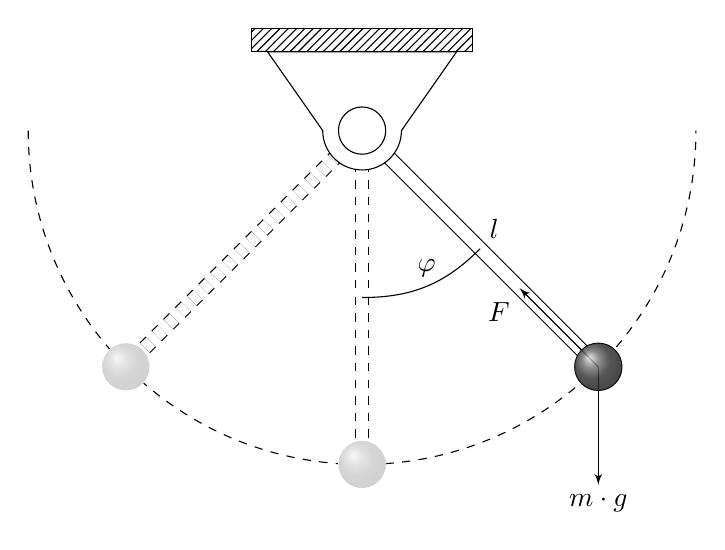
\begin{tikzpicture}[auto, >=latex']

    \draw[dashed] (-4.24,0) arc (-180:0:4.24);

    \coordinate (l) at (-3,-3);
    \coordinate (m) at (0,-4.24);
    \coordinate (r) at (3,-3);

    % left
    \draw[double distance=1.6mm,dashed] (0,0) -- (l);
    \draw[draw=white,fill=white] (l) circle (.3cm);

    % middle
    \draw[double distance=1.6mm,dashed] (0,0) -- (m);
    \draw[draw=white,fill=white] (m) circle (.3cm);

    % right
    \draw[double distance=1.6mm] (0,0) -- node [midway] {$l$} (r);
    \draw[draw=black,fill=white] (r) circle (.3cm);
    \draw[->] (3,-3) -- (3,-4.5) node[below]{$m\cdot g$};

    \draw[-] ($(m)!0.5!(0,0)$) to [bend right=22.5] node [above] {$\varphi$} ($(r)!0.5!(0,0)$);

    \draw[fill=white] (-1.2,1.0) -- (-.5,0) arc(180:360:0.5) -- (1.2,1.0) -- cycle;
    \draw[draw=black,fill=white] (0, 0) circle (.3cm);
    \draw[pattern=north east lines] (-1.4,1.3) rectangle (1.4,1);
    \draw[->] (3,-3) -- (2.,-2.0) node[left,yshift=-3mm]{$F$};

    \shade[ball color=black!75!white,opacity=0.20] (l) circle (0.3cm);
    \shade[ball color=black!75!white,opacity=0.20] (m) circle (0.3cm);
    \shade[ball color=black!75!white,opacity=0.80] (r) circle (0.3cm);

\end{tikzpicture}

    % Steuerung
%	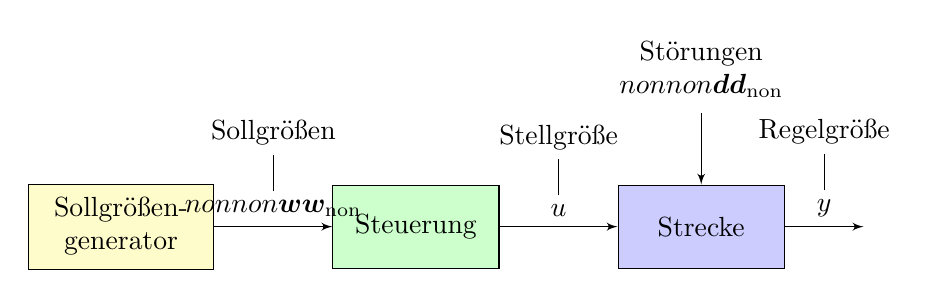
\begin{tikzpicture}[auto, >=latex']

    \node [block, minimum width=6em, fill=yellow!20] (sollgroesse) {\begin{tabular}{c}Sollgrößen-\\generator\end{tabular}};
    \node [block, minimum width=6em, fill=green!20, node distance=1.5cm, right=of sollgroesse] (steuerung) {Steuerung};
    \node [block, minimum width=6em, fill=blue!20, node distance=1.5cm, right=of steuerung,
    pin={[pin distance=6ex, pinstyle]above:\begin{tabular}{c}Störungen\\$\bmd$\end{tabular}}] (regelstrecke) {Strecke};
	\node [output, node distance=1cm, right= of regelstrecke] (x) {};

    \draw [->] (sollgroesse) -- node [above, pin={[pin edge={-, thin, black}]90:Sollgrößen}] {$\bmw$} (steuerung);
    \draw [->] (steuerung) -- node [above, pin={[pin edge={-, thin, black}]90:Stellgröße}] {$u$} (regelstrecke);
    \draw [->] (regelstrecke) -- node [above, pin={[pin edge={-, thin, black}]90:Regelgröße}] {$y$} (x);

\end{tikzpicture}

    % Regelung
%	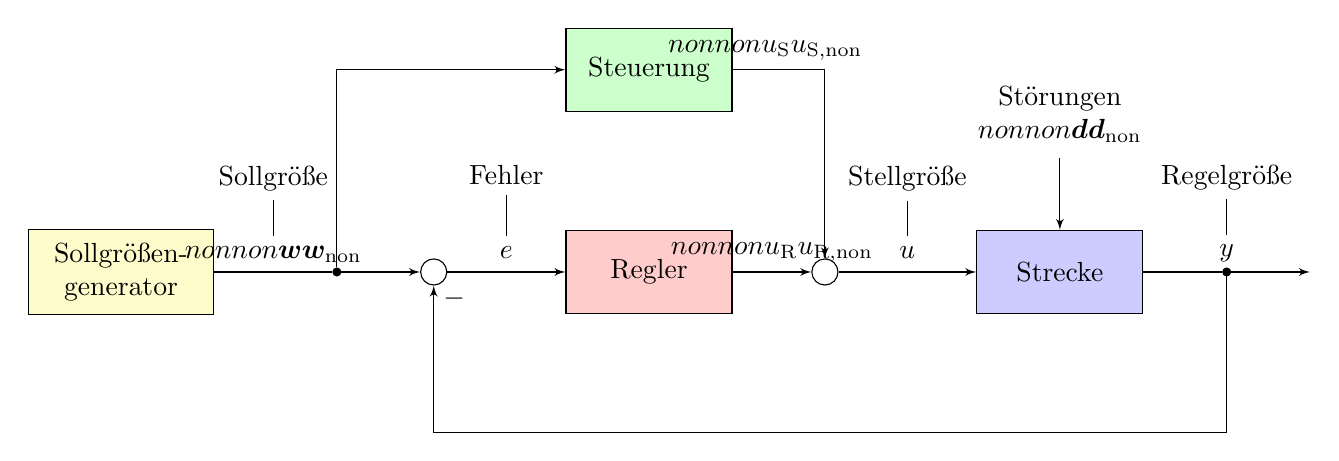
\begin{tikzpicture}[auto, >=latex']

	\node [block, minimum width=6em, fill=yellow!20] (sollgroesse)
	{\begin{tabular}{c}Sollgrößen-\\generator\end{tabular}};
	\node [branch, node distance=1.5cm, right=of sollgroesse] (brFF) {};
	\node [sum, node distance=1cm, right=of brFF] (sumerror) {};
	\node [block, minimum width=6em, fill=red!20, node distance=1.5cm, right=of sumerror] (regler) {Regler};
	\node [block, minimum width=6em, fill=green!20, node distance=1.5cm, above=of regler] (steuerung) {Steuerung};
    \node [sum, node distance=1cm, right=of regler] (sumFF) {};
	\node [block, minimum width=6em, fill=blue!20, node distance=1.75cm, right=of sumFF, pin={[pin distance=6ex, pinstyle]above:\begin{tabular}{c}Störungen\\$\bmd$\end{tabular}}] (regelstrecke)
		{Strecke};
	\node [branch, node distance=1cm, right=of regelstrecke] (bx) {};
	\node [output, node distance=1cm, right= of bx] (x) {};
	\node [coord, node distance=1.5cm, below=of regler] (rueckfuehrung) {};

	\draw [-] (sollgroesse) -- node [above, pin={[pin edge={-, thin, black}]90:Sollgröße}] {$\bmw\vphantom{_{\mathrm{R}}}$} (brFF);
    \draw [->] (brFF) -- (sumerror);
    \draw [->] (sumerror) -- node [above, pin={[pin distance=3.5ex, pin edge={-, thin, black}]90:Fehler}] {$e\vphantom{_{\mathrm{R}}}$}
	(regler);
    \draw [->] (regler) -- node [above] {$\uR$} (sumFF);
    \draw [->] (sumFF) -- node [above, pin={[pin edge={-, thin, black}]90:Stellgröße}]
	{$u\vphantom{_{\mathrm{R}}}$} (regelstrecke);
	\draw [-] (regelstrecke) -- (bx) node [above, pin={[pin edge={-, thin, black}]90:Regelgröße}] {$y\vphantom{_{\mathrm{R}}}$};
	\draw [->] (bx) -- (x);
	\draw [-] (bx) |- (rueckfuehrung);
	\draw [->] (rueckfuehrung) -| node[right, yshift=1.7cm] {$-$} (sumerror);
    \draw [->] (brFF) |- (steuerung);
	\draw [->] (steuerung) node [above, xshift=9.75ex] {$\uS$} -| (sumFF);

\end{tikzpicture}

    % Zweitanksystem
%	\tikzset{
    waterIn1/.pic={
        \fill[cyan!25](-2.5, -0.25) rectangle (0.25, 0.25);
        \draw[dashed, color=gray, line width=1pt] (-0.4, 0.25) arc (-90:90:0.125 and -0.25);
        \draw[color=gray, line width=1pt] (-0.4, -0.25) arc (90:270:0.125 and -0.25);
        \draw[line width=1pt](-2.5, -0.25) -- (0.25, -0.25) (-2.5, 0.25) -- (0.25, 0.25);
        \node at (-0.4, -0.6) {$\Ain[1]$};
    },
    waterIn2/.pic={
        \fill[cyan!25](-1.0, -0.25) rectangle (0.25, 0.25);
        \draw[dashed, color=gray, line width=1pt] (-0.4, 0.25) arc (-90:90:0.125 and -0.25);
        \draw[color=gray, line width=1pt] (-0.4, -0.25) arc (90:270:0.125 and -0.25);
        \draw[line width=1pt](-1.0, -0.25) -- (0.25, -0.25) (-1.0, 0.25) -- (0.25, 0.25);
        \node at (-0.4, -0.65) {$\Ain[2]$};
    },
    waterOut1/.pic={
        \fill[cyan!25](-1.00, -0.25) rectangle (0.25, 0.25);
        \fill[cyan!25](-1.00, -0.25) rectangle (-0.50, -1.5);
        \draw[dashed, color=gray, line width=1pt] (-0.5, -0.75) arc (0:180:0.25 and -0.125);
        \draw[color=gray, line width=1pt] (-1, -0.75) arc (180:0:0.25 and 0.125);
        \draw[line width=1pt](0.25, -0.25) -- (-0.5, -0.25) -- (-0.5, -1.5) (0.25, 0.25) -- (-1.00, 0.25) -- (-1.00, -1.5);
        \node at (-1.4, -0.75) {$\Aout[1]$};
    },
    waterOut2/.pic={
        \fill[cyan!25](-1.00, -0.25) rectangle (0.25, 0.25);
        \fill[cyan!25](-1.00, -0.25) rectangle (-0.50, -3.5);
        \draw[dashed, color=gray, line width=1pt] (-0.5, -0.75) arc (0:180:0.25 and -0.125);
        \draw[color=gray, line width=1pt] (-1, -0.75) arc (180:0:0.25 and 0.125);
        \draw[line width=1pt](0.25, -0.25) -- (-0.5, -0.25) -- (-0.5, -3.5) (0.25, 0.25) -- (-1.00, 0.25) -- (-1.00, -3.5);
        \node at (-1.4, -0.75) {$\Aout[2]$};
    },
    pumpe/.style={
        circle,
        fill=white,
        draw,
        thick,
        minimum size=1cm,
        path picture={
        \draw [thick] (path picture bounding box.north) --
                      (path picture bounding box.east) --
                      (path picture bounding box.south);
        },
    },
    ventil/.pic={
        \fill[white] (0.4, 0) rectangle (-0.4, -1.2);
        \draw[line width=1pt] (-0.4, 0) -- (0.4, 0) -- (-0.4, -1.2) -- (0.4, -1.2) -- cycle;
    },
}
\begin{tikzpicture}[auto, >=latex']

    \begin{scope}
        \fill[cyan!25] decorate[decoration={random steps, segment length=1mm, amplitude=0.5mm}]{(6, 2.2) -- (0, 2.2)}--(0,0) -- (6, 0) -- cycle;
        \draw[line width=1pt] (0,0) rectangle (6, 4);

        \coordinate (eingang) at (0, 4.0 - 0.7);
        \coordinate (ausgang) at (6.0 - 1.0, 0);

        \pic[xshift=-2.5mm + 0.5pt] at (eingang) {waterIn1};
        \pic[xshift=2.5mm - 0.5pt, rotate=90] at (ausgang) {waterOut1};

        \fill[cyan!25] ([shift={(0.5pt, -2.5mm)}]eingang) parabola (0.3 * 6, 1pt) -- (0.5 * 6, 1pt) parabola[bend at end] ([shift={(0.5pt, 2.5mm)}]eingang);

        \draw[thick] (-1.5, 4.0 - 0.7) -- (-1.5, 4.4);
        \draw[thick] (-2.0, 4.0 - 0.7) -- (-2.0, 4.4);
        \draw[thick] (-1.5, 4.5) circle (0.1);
        \draw[thick] (-2, 4.5) circle (0.1);
        \draw (-1.5, 4.5) node [right] {$+$};
        \draw (-2, 4.5) node [left] {$-$};

        \draw[->] (-1.5, 4.7) to [out=130, in=50] node [above] {\large $\uA$} (-2, 4.7);

        \node[pumpe] at (-1.75, 4.0 - 0.7) () {};

        \draw[|-|] (6.3, 0) -- node[fill=white, inner xsep=0, xshift=1.5mm] {$h$} (6.3, 4);
        \draw[|->|] (-0.3, 0) -- node[fill=white, inner xsep=0, xshift=2mm] {$z_1$} (-0.3, 2.2);
        \draw[|-|] (0, 4.3) -- node[fill=white, inner xsep=0, yshift=-2.9mm] {$\AT[1]$} (6, 4.3);
        \draw[|-|] (5 - 0.3, 0) -- node[fill=white, inner xsep=0, xshift =-4.6mm] {$\hvb[1]$} (5 - 0.3, -1);

        \draw[->] ([shift={(-32.5mm, 0)}]eingang) node [left] {$\Vdin[1]$} --  ([shift={(-27.5mm, 0)}]eingang);
        \draw[->] ([shift={(37.5mm, -7.55mm)}]ausgang) --  ([shift={(42.5mm, -7.55mm)}]ausgang);

        \draw[->] (11.5, 3.5) -- node [right] {$g$} (11.5, 1.5);
    \end{scope}

    \begin{scope}[shift={(85mm, -40.5mm)}]
        \fill[cyan!25] decorate[decoration={random steps, segment length=1mm, amplitude=0.5mm}]{(6, 2.2) -- (0, 2.2)}--(0,0) -- (6, 0) -- cycle;
        \draw[line width=1pt] (0,0) rectangle (6, 4);

        \coordinate (eingang) at (0, 4.0 - 0.7);
        \coordinate (ausgang) at (6.0 - 1.0, 0);

        \pic[xshift=-2.5mm + 0.5pt] at (eingang) {waterIn2};
        \pic[xshift=2.5mm - 0.5pt, rotate=90] at (ausgang) {waterOut2};

        \fill[cyan!25] ([shift={(0.5pt, -2.5mm)}]eingang) parabola (0.3 * 6, 1pt) -- (0.5 * 6, 1pt) parabola[bend at end] ([shift={(0.5pt, 2.5mm)}]eingang);

        \pic[xshift=-21.5mm, rotate=90] at (eingang) {ventil};

        \pic[xshift=90pt, yshift=-21.5pt, rotate=-90] at (ausgang) {ventil};

        \draw[|-|] (6.3, 0) -- node[fill=white, inner xsep=0, xshift=1.5mm] {$h$} (6.3, 4);
        \draw[|->|] (-0.3, 0) -- node[fill=white, inner xsep=0, xshift=2mm] {$z_2$} (-0.3, 2.2);
        \draw[|-|] (0, 4.3) -- node[fill=white, inner xsep=0, yshift=-2.9mm] {$\AT[2]$} (6, 4.3);
        \draw[|-|] (5 - 0.3, 0) -- node[fill=white, inner xsep=0, xshift =-4.6mm] {$\hvb[2]$} (5 - 0.3, -1);

        \draw[->] ([shift={(37.5mm, -7.55mm)}]ausgang) -- ([shift={(42.5mm, -7.55mm)}]ausgang) node [right] {$\Vdout[2]$};

        \draw[->] ([shift={(-20mm, 6mm)}]eingang) -- node [above] {$\Vd[1,2]$} ([shift={(-10mm, 6mm)}]eingang);
    \end{scope}

\end{tikzpicture}

    % HVAC
%	\tikzset{
    Heat/.style={
         draw=none,
         inner color=red,
         outer color=yellow,
            postaction={
                decorate,
                rounded corners=2pt,
                decoration={
                    markings,
                    mark=between positions 6pt and 55pt step 9pt
                    with {
                        \draw[-Triangle,red,line width=0.5pt](0,0)
                            --++(0.1,0.1)
                            --++(-0.2,0.1)
                            --++(0.1,0.1)
                            --++(0,0.2);
                    }
                }
            }
    },
    Cool/.style={
         draw=none,
            postaction={
                decorate,
                rounded corners=2pt,
                decoration={
                    markings,
                    mark=between positions 6pt and 55pt step 9pt
                    with {
                        \draw[-Triangle,blue,line width=0.5pt](0,0)
                            --++(0.1,0.1)
                            --++(-0.2,0.1)
                            --++(0.1,0.1)
                            --++(0,0.2);
                    }
                }
            }
      },
    CoolHeat/.style={
         draw=none,
            postaction={
                decorate,
                rounded corners=2pt,
                decoration={
                    markings,
                    mark=between positions 6pt and 55pt step 9pt
                    with {
                        \draw[-Triangle,blue!50!red,line width=0.5pt](0,0)
                            --++(0.1,0.1)
                            --++(-0.2,0.1)
                            --++(0.1,0.1)
                            --++(0,0.2);
                    }
                }
            }
      },
}

\begin{tikzpicture}[auto, >=latex', circuit pid ISO14617, every info/.style={font=\tiny}]

    \draw [thick] (0, -0.1) -- (6, -0.1);
    \draw [thick] (0, 1.775) -- (6, 1.775);
    \node [fan, circuit symbol unit=21pt] at (4, 0.8375) () {};

    \draw [Heat, rotate=-90] (-1.375, 2) -- ++(0,4pt) -- ++(30pt,0) -- ++(0,-4pt);
    \draw [Cool, rotate=-90] (-1.7, 0) -- ++(0,4pt) -- ++(50pt,0) -- ++(0,-4pt);
    \draw [CoolHeat, rotate=-90] (-1.7, 5.25) -- ++(0,4pt) -- ++(50pt,0) -- ++(0,-4pt);

    \draw[thick] (3.6, 0.01) -- (3.6, -0.4);
    \draw[thick] (4.4, 0.01) -- (4.4, -0.4);
    \draw[thick] (4.4, -0.5) circle (0.1);
    \draw[thick] (3.6, -0.5) circle (0.1);
    \draw (4.4, -0.5) node [right] {$+$};
    \draw (3.6, -0.5) node [left] {$-$};

    \draw[thick] (1.2, -0.4) -- (1.2, 0.9) -- (1.6, 0.9) -- (1.8, 1.2) -- (2, 1.4);
    \draw[thick] (1.5, -0.4) -- (1.5, 0.8) -- (1.6, 0.8) -- (1.8, 0.5) -- (2, 0.3);
    \draw[thick] (1.5, -0.5) circle (0.1);
    \draw[thick] (1.2, -0.5) circle (0.1);
    \draw (1.5, -0.5) node [right] {$+$};
    \draw (1.2, -0.5) node [left] {$-$};
\end{tikzpicture}

    % Tankkaskade
%	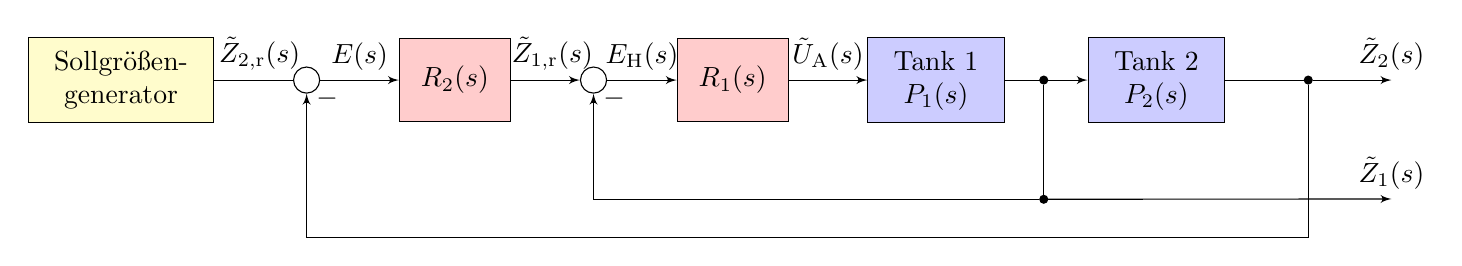
\begin{tikzpicture}[auto, >=latex']
	\node [block, minimum width=6em, fill=yellow!20] (sollgroesse)
	{\begin{tabular}{c}Sollgrößen-\\generator\end{tabular}};
	\node [sum, node distance=1cm, right=of sollgroesse] (sumerror) {};
	\node [block, minimum width=4em, fill=red!20, right=of sumerror] (cont1)
		{$R_2(s)$};
	\node [coord, node distance=2cm, below of= cont1] (rueckfuehrung) {};
	\node [block, minimum width=4em, node distance=6em, fill=red!20, right=of cont1] (cont2)
		{$R_1(s)$};
	\node [block, minimum width=4em, right=of cont2,fill=blue!20] (sysDyn)
    {\begin{tabular}{c} Tank 1\\$P_1(s)$\end{tabular}};
	\node [sum, node distance=2.5em, right=of cont1] (sumH) {};
	\node [block, minimum width=4em, node distance=3em, right=of sysDyn, fill=blue!20]
			(sysDyn2) {\begin{tabular}{c} Tank 2\\$P_2(s)$\end{tabular}};
	\node [branch, node distance=1cm, right=of sysDyn2] (bx) {};
	\node [output, node distance=1cm, right= of bx] (x) {};
	\node [output, node distance=1.51cm, below= of x] (xH) {};
	\node [branch, node distance=1.25em, right=of sysDyn] (byH) {};
	\node [branch, node distance=1.4cm, below=of byH] (byEH) {};

    \draw [-] (sollgroesse) -- node [above,xshift=0.5ex] {$\tilde{Z}_{2,\mathrm{r}}(s)$} (sumerror);
	\draw [->] (sumerror) -- node [above] {$E(s)$} (cont1);
    \draw [->] (cont2) -- node [above] {$\tilde{U}_{\mathrm{A}}(s)$} (sysDyn);
	\draw [-] (sysDyn2) -- (bx);
    \draw [->] (bx) -- (x) node [above] {$\tilde{Z}_2(s)$};
	\draw [->] (bx) |-  (rueckfuehrung) -| (sumerror) node[below right] {$-$};
	\draw [->] (sysDyn) -- (sysDyn2);
    \draw [->] (byEH) -- (xH) node [above] {$\tilde{Z}_1(s)$};
    \draw [-] (byH) -- (byEH);
    \draw [->] (cont1) -- node[above, xshift=.25em] {$\tilde{Z}_\mathrm{1,r}(s)$} (sumH);
	\draw [->] (sumH) -- node[above] {$E_\mathrm{H}(s)$} (cont2);
	\draw [->] (byEH) -| (sumH) node[below right] {$-$};
\end{tikzpicture}

    % Smith-Prädiktor
%	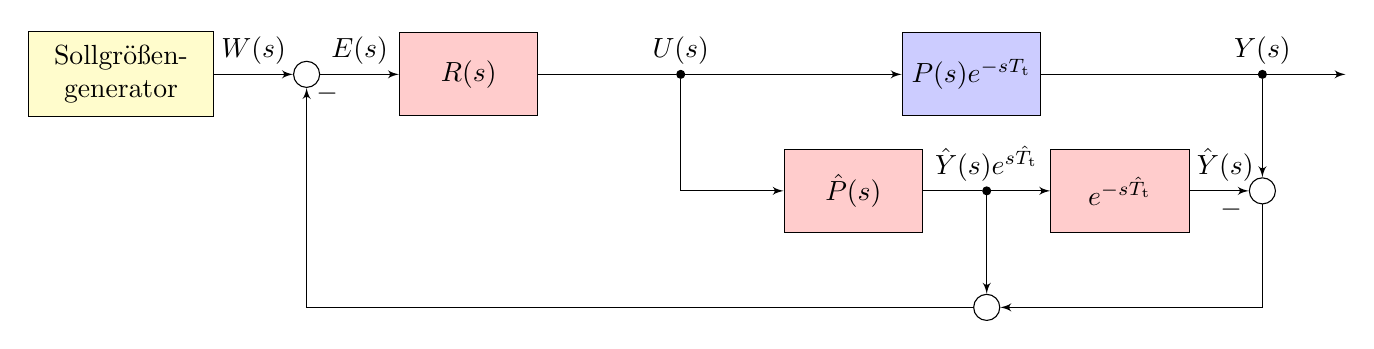
\begin{tikzpicture}[auto, >=latex']
	\node [block, minimum width=6em, fill=yellow!20] (sollgroesse)
	{\begin{tabular}{c}Sollgrößen-\\generator\end{tabular}};
	\node [sum, node distance=1cm, right=of sollgroesse] (sumerror) {};
	\node [block, minimum width=5em, node distance=1cm, fill=red!20, right=of sumerror] (regler) {$R(s)$};
	\node [branch, node distance=1.75cm, right=of regler] (bR) {};
    \node [block, minimum width=5em, node distance=2.75cm, fill=blue!20, right=of bR] (process) {$P(s)e^{-s T_\mathrm{t}}$};
	\node [branch, node distance=2.75cm, right=of process] (bP) {};
    \node [output, node distance=1cm, right= of bP] (x) {};

	\node [sum, node distance=1.25cm, below=of bP] (sumDelay) {};
    \node [block, minimum width=5em, node distance=0.75cm, fill=red!20, left=of sumDelay] (delay) {$e^{-s \hat{T}_\mathrm{t}}$};
	\node [branch, node distance=0.75cm, left=of delay] (bD) {};
    \node [block, minimum width=5em, node distance=0.75cm, fill=red!20, left=of bD] (g) {$\hat{P}(s)$};
	\node [sum, node distance=1.25cm, below=of bD] (sumSmith) {};

    \draw [->] (sollgroesse) -- node [above] {$W(s)$} (sumerror);
    \draw [->] (sumerror) -- node [above] {$E(s)$} (regler);
    \draw [->] (regler) -- (bR) node [above] {$U(s)$} -- (process);
    \draw [->] (process) -- (bP) node [above] {$Y(s)$} -- (x);
    \draw [->] (bR) |- (g);
    \draw [->] (g) -- (bD) node [above] {$\hat{Y}(s) e^{s \hat{T}_\mathrm{t}} $} -- (delay);
    \draw [->] (bD) -- (sumSmith);
    \draw [->] (sumSmith) -| (sumerror) node [below right] {$-$};
    \draw [->] (bP) -- (sumDelay);
    \draw [->] (delay) -- node [below, xshift=1ex] {$-$} node [above, xshift=0.5ex] {$\hat{Y}(s)$} (sumDelay);
    \draw [->] (sumDelay) |- (sumSmith);

\end{tikzpicture}

\end{document}
